\section{Algoritmo di Hoshen-Kopelman}
L’algoritmo di Hoshen-Kopelman (HK76) è una tecnica di etichettatura multipla dei cluster. Il reticolo viene visitato sito per sito per colonne, partendo dallo spigolo in alto a sinistra per arrivare a quello in basso a destra. Si prenda, ad esempio, il reticolo
in figura
\begin{figure}[H]
	\centering
	\scriptsize % Riduce la dimensione del testo
	\setlength{\tabcolsep}{5.4pt} % Riduce lo spazio tra le colonne
	\renewcommand{\arraystretch}{1.3} % Riduce lo spazio verticale tra le righe
	\begin{minipage}{0.45\textwidth}
		\centering
		\begin{tabular}{|*{15}{c|}}
			\hline
			0 & 1 & 0 & 0 & 1 & 1 & 0 & 0 & 0 & 1 & 0 & 1 & 0 & 1 & 0 \\
			\hline
			0 & 1 & 1 & 0 & 0 & 0 & 1 & 0 & 0 & 1 & 1 & 1 & 1 & 1 & 1 \\
			\hline
			0 & 1 & 0 & 0 & 0 & 1 & 1 & 1 & 1 & 0 & 0 & 1 & 0 & 0 & 0 \\
			\hline
			1 & 0 & 1 & 0 & 1 & 0 & 1 & 0 & 0 & 0 & 1 & 1 & 0 & 0 & 0 \\
			\hline
			0 & 1 & 0 & 1 & 1 & 0 & 1 & 0 & 0 & 0 & 1 & 0 & 0 & 1 & 0 \\
			\hline
			0 & 0 & 1 & 1 & 1 & 1 & 1 & 0 & 1 & 1 & 1 & 1 & 1 & 0 & 1 \\
			\hline
			0 & 0 & 1 & 1 & 1 & 0 & 0 & 0 & 0 & 1 & 1 & 1 & 1 & 0 & 1 \\
			\hline
			0 & 1 & 0 & 1 & 1 & 1 & 1 & 0 & 1 & 1 & 1 & 1 & 0 & 1 & 0 \\
			\hline
			0 & 1 & 0 & 0 & 1 & 1 & 0 & 0 & 1 & 1 & 1 & 1 & 0 & 0 & 1 \\
			\hline
			1 & 0 & 0 & 0 & 0 & 0 & 0 & 0 & 1 & 0 & 0 & 0 & 0 & 1 & 0 \\
			\hline
			0 & 0 & 0 & 0 & 1 & 0 & 1 & 0 & 1 & 1 & 0 & 1 & 1 & 1 & 1 \\
			\hline
			1 & 1 & 0 & 0 & 0 & 1 & 0 & 1 & 0 & 1 & 1 & 1 & 1 & 1 & 1 \\
			\hline
			1 & 1 & 1 & 0 & 0 & 1 & 1 & 0 & 1 & 0 & 0 & 1 & 0 & 0 & 0 \\
			\hline
			0 & 1 & 0 & 1 & 1 & 1 & 1 & 1 & 0 & 1 & 1 & 1 & 0 & 1 & 1 \\
			\hline
			1 & 1 & 1 & 1 & 0 & 0 & 0 & 0 & 1 & 1 & 1 & 1 & 1 & 1 & 0 \\
			\hline
		\end{tabular}
	\end{minipage}
	\hfill
	\begin{minipage}{0.45\textwidth}
		\centering
		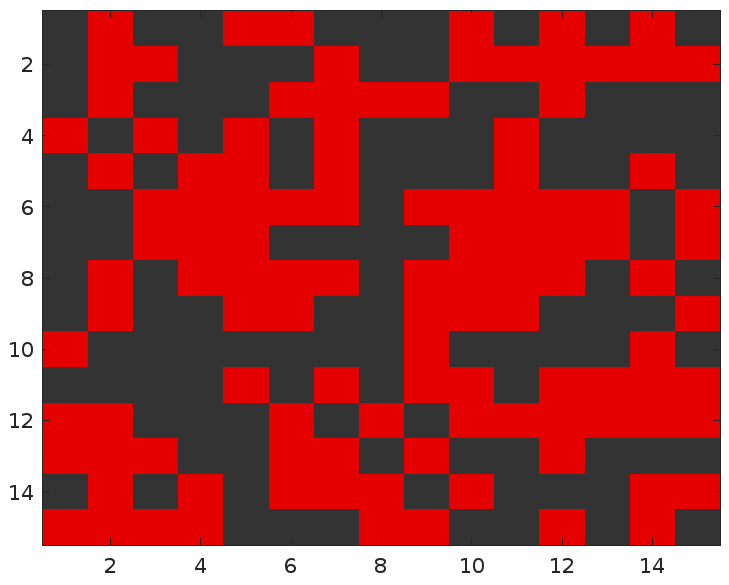
\includegraphics[width=\linewidth]{images/basegrid}
		\label{fig:basegrid}
	\end{minipage}
\end{figure}
\noindent
Durante la visita del reticolo, quando si incontra un sito colorato, allora: \textbf{(1)} Se il sito non è connesso ad altri siti colorato sopra o a sinistra, si inizia un nuovo cluster, a cui viene assegnata una \texttt{label} \textbf{(2)} Se c’è un primo vicino sopra o a sinistra colorato (uno solo dei due), il sito viene aggiunto al cluster del primo vicino colorato \textbf{(3)}Se i suoi primi vicini sono entrambi colorati, ma appartengono allo stesso cluster, il sito viene aggiunto al cluster dei primi vicini \textbf{(4)} Se i suoi primi vicini sono entrambi colorati, e non appartengono allo stesso cluster, il sito viene aggiunto al cluster con la \texttt{label} minore. Ad esempio, il cluster associati al reticolo precedente sono
mostrati in figura
\begin{figure}[H]
	\centering
	\scriptsize % Riduce la dimensione del testo
	\setlength{\tabcolsep}{3.5pt} % Riduce lo spazio tra le colonne
	\renewcommand{\arraystretch}{1.3} % Riduce lo spazio verticale tra le righe
	\begin{minipage}{0.4\textwidth}
		\centering
		\begin{center}
			\begin{tabular}{|*{15}{c|}}
				\hline
				0 & 1 & 0 & 0 & 2 & 2 & 0 & 0 & 0 & 3 & 0 & 4 & 0 & 5 & 0 \\
				\hline
				0 & 1 & 1 & 0 & 0 & 0 & 6 & 0 & 0 & 3 & 3 & 3 & 3 & 3 & 3 \\
				\hline
				0 & 1 & 0 & 0 & 0 & 7 & 6 & 6 & 6 & 0 & 0 & 3 & 0 & 0 & 0 \\
				\hline
				8 & 0 & 9 & 0 & 10 & 0 & 6 & 0 & 0 & 0 & 11 & 3 & 0 & 0 & 0 \\
				\hline
				0 & 12 & 0 & 13 & 10 & 0 & 6 & 0 & 0 & 0 & 11 & 0 & 0 & 14 & 0 \\
				\hline
				0 & 0 & 15 & 13 & 10 & 10 & 6 & 0 & 16 & 16 & 11 & 11 & 11 & 0 & 17 \\
				\hline
				0 & 0 & 15 & 13 & 10 & 0 & 0 & 0 & 0 & 16 & 11 & 11 & 11 & 0 & 17 \\
				\hline
				0 & 18 & 0 & 13 & 10 & 10 & 10 & 0 & 19 & 16 & 11 & 11 & 0 & 20 & 0 \\
				\hline
				0 & 18 & 0 & 0 & 10 & 10 & 0 & 0 & 19 & 16 & 11 & 11 & 0 & 0 & 21 \\
				\hline
				22 & 0 & 0 & 0 & 0 & 0 & 0 & 0 & 19 & 0 & 0 & 0 & 0 & 23 & 0 \\
				\hline
				0 & 0 & 0 & 0 & 24 & 0 & 25 & 0 & 19 & 19 & 0 & 26 & 26 & 23 & 23 \\
				\hline
				27 & 27 & 0 & 0 & 0 & 28 & 0 & 29 & 0 & 19 & 19 & 19 & 19 & 19 & 19 \\
				\hline
				27 & 27 & 27 & 0 & 0 & 28 & 28 & 0 & 30 & 0 & 0 & 19 & 0 & 0 & 0 \\
				\hline
				0 & 27 & 0 & 31 & 31 & 28 & 28 & 28 & 0 & 32 & 32 & 19 & 0 & 33 & 33 \\
				\hline
				34 & 27 & 27 & 27 & 0 & 0 & 0 & 0 & 35 & 32 & 32 & 19 & 19 & 19 & 0 \\
				\hline
			\end{tabular}
		\end{center}
	\end{minipage}
	\hfill
	\begin{minipage}{0.45\textwidth}
		\centering
		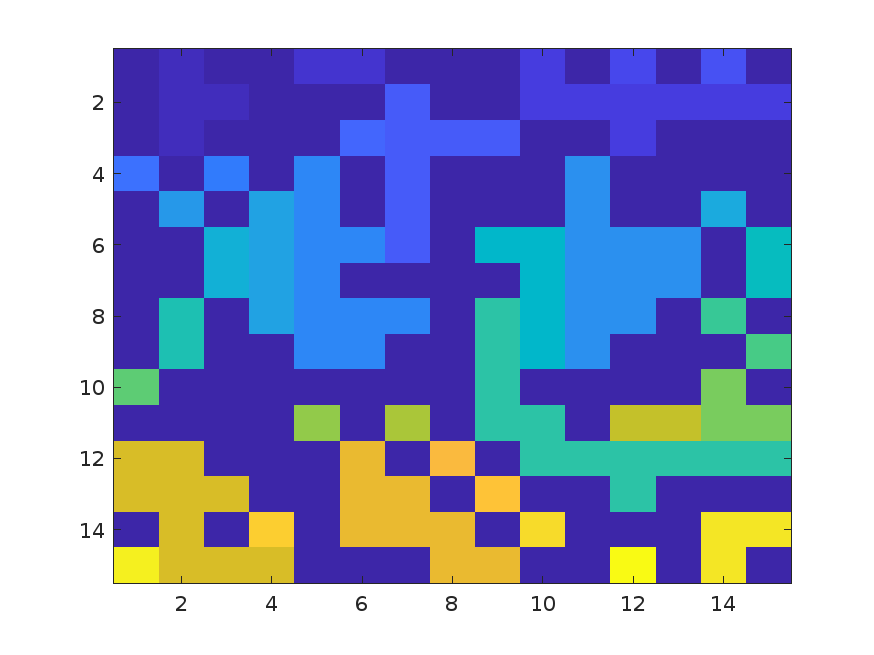
\includegraphics[width=\linewidth]{images/labels}
		\label{fig:basegrid}
	\end{minipage}
\end{figure}
\noindent
Tuttavia, quando si incontra un caso come quello descritto nel punto \textbf{(4)}, occorre  memorizzare che i due cluster sono in realtà lo stesso cluster. Questo viene fatto usando un vettore chiamato \textbf{Label of Label} (\texttt{LofL}), che contiene tutta l’informazione necessaria sui label dei cluster. In particolare, il modulo \texttt{HKclass}: 
per un \textit{good label}, memorizza la taglia del cluster; 
per \textit{bad label}, memorizza qual è il vero cluster label a cui questo label appartiene.  Questa distinzione viene fatta attraverso i segni dei numeri interi contenuti in LofL. Di seguito è riportato il LofL corrispondete al reticolo preso in esame

\vspace{15px}
\noindent
\begin{tabular}{|c|*{12}{c|}}
	\hline
	\textbf{ID}   & 1 & 2 & 3 & 4 & 5 & 6 & 7 & 8 & 9 & 10 & 11 & 12 \\
	\hline
	\textbf{Val}  & 4 & 2 & 56 & -3 & -3 & 24 & -6 & 1 & 1 & -6 & -3 & 1 \\
	\hline
\end{tabular}

\vspace{10px}
\noindent
\begin{tabular}{|c|*{12}{c|}}
	\hline
	\textbf{ID}   & 13 & 14 & 15 & 16 & 17 & 18 & 19 & 20 & 21 & 22 & 23 & 24 \\
	\hline
	\textbf{Val}  & -10 & 1 & -10 & -3 & 2 & 2 & -3 & 1 & 1 & 1 & -3 & 1 \\
	\hline
\end{tabular}

\vspace{10px}
\noindent
\begin{tabular}{|c|*{11}{c|}}
	\hline
	\textbf{ID}   & 25 & 26 & 27 & 28 & 29 & 30 & 31 & 32 & 33 & 34 & 35 \\
	\hline
	\textbf{Val}  & 1 & -3 & 18 & -27 & 1 & 1 & -27 & -3 & -3 & -27 & -3 \\
	\hline
\end{tabular}

\vspace{15px}
\noindent
Tuttavia, l’algoritmo HK restituisce in modo corretto le taglie dei cluster, ma non garantisce che tutti i siti di un fissato cluster abbiano lo stesso valore. Per questo motivo, al fine di identificare la presenza di cluster percolanti, effettuiamo una rilabelizzazione successiva. Di seguito ne è mostrato un esempio.

\begin{figure}[H]
	\centering
	\scriptsize % Riduce la dimensione del testo
	\setlength{\tabcolsep}{3.5pt} % Riduce lo spazio tra le colonne
	\renewcommand{\arraystretch}{1.3} % Riduce lo spazio verticale tra le righe
	\begin{minipage}{0.4\textwidth}
		\centering
		\begin{center}
			\begin{tabular}{|*{15}{c|}}
				\hline
				0 & 1 & 0 & 0 & 2 & 2 & 0 & 0 & 0 & 3 & 0 & 3 & 0 & 3 & 0 \\
				\hline
				0 & 1 & 1 & 0 & 0 & 0 & 6 & 0 & 0 & 3 & 3 & 3 & 3 & 3 & 3 \\
				\hline
				0 & 1 & 0 & 0 & 0 & 6 & 6 & 6 & 6 & 0 & 0 & 3 & 0 & 0 & 0 \\
				\hline
				8 & 0 & 9 & 0 & 6 & 0 & 6 & 0 & 0 & 0 & 3 & 3 & 0 & 0 & 0 \\
				\hline
				0 & 12 & 0 & 6 & 6 & 0 & 6 & 0 & 0 & 0 & 3 & 0 & 0 & 14 & 0 \\
				\hline
				0 & 0 & 6 & 6 & 6 & 6 & 6 & 0 & 3 & 3 & 3 & 3 & 3 & 0 & 17 \\
				\hline
				0 & 0 & 6 & 6 & 6 & 0 & 0 & 0 & 0 & 3 & 3 & 3 & 3 & 0 & 17 \\
				\hline
				0 & 18 & 0 & 6 & 6 & 6 & 6 & 0 & 3 & 3 & 3 & 3 & 0 & 20 & 0 \\
				\hline
				0 & 18 & 0 & 0 & 6 & 6 & 0 & 0 & 3 & 3 & 3 & 3 & 0 & 0 & 21 \\
				\hline
				22 & 0 & 0 & 0 & 0 & 0 & 0 & 0 & 3 & 0 & 0 & 0 & 0 & 3 & 0 \\
				\hline
				0 & 0 & 0 & 0 & 24 & 0 & 25 & 0 & 3 & 3 & 0 & 3 & 3 & 3 & 3 \\
				\hline
				27 & 27 & 0 & 0 & 0 & 27 & 0 & 29 & 0 & 3 & 3 & 3 & 3 & 3 & 3 \\
				\hline
				27 & 27 & 27 & 0 & 0 & 27 & 27 & 0 & 30 & 0 & 0 & 3 & 0 & 0 & 0 \\
				\hline
				0 & 27 & 0 & 27 & 27 & 27 & 27 & 27 & 0 & 3 & 3 & 3 & 0 & 3 & 3 \\
				\hline
				27 & 27 & 27 & 27 & 0 & 0 & 0 & 0 & 3 & 3 & 3 & 3 & 3 & 3 & 0 \\
				\hline
			\end{tabular}
		\end{center}
	\end{minipage}
	\hfill
	\begin{minipage}{0.45\textwidth}
		\centering
		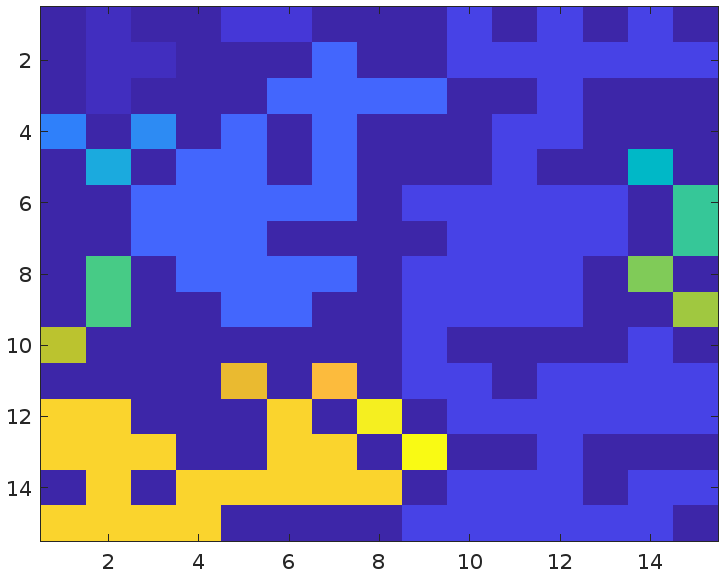
\includegraphics[width=\linewidth]{images/re-labelled}
		\label{fig:basegrid}
	\end{minipage}
\end{figure}
\noindent
A questo punto, l'obiettivo è determinare se esistono cluster percolanti all'interno del reticolo, ossia se esiste almeno un'etichetta condivisa tra la prima e l'ultima riga (percolazione verticale) e tra la prima e l'ultima colonna (percolazione orizzontale). Per fare ciò, possiamo sviluppare un algoritmo che, basandosi sull'estrazione delle etichette \textbf{uniche} presenti lungo i bordi della matrice, e mediante l'utilizzo dell'operazione \texttt{intersect},  verifica l'esistenza di almeno una etichetta comune tra i bordi opposti. Se tale etichetta è presente, viene restituito \texttt{true} per il tipo di percolazione considerato, altrimenti \texttt{false}.
\\\\
\noindent
Tuttavia, poiché ci interessa esclusivamente determinare il cluster di appartenenza della prima e dell’ultima riga e colonna per valutare la percolazione, è sufficiente rilabelare solo questi elementi, ignorando il centro del reticolo e risparmiando così tempo di calcolo. La Figura \ref{fig:relabelled-edge} ne mostra un esempio.
\begin{figure}
	\centering
	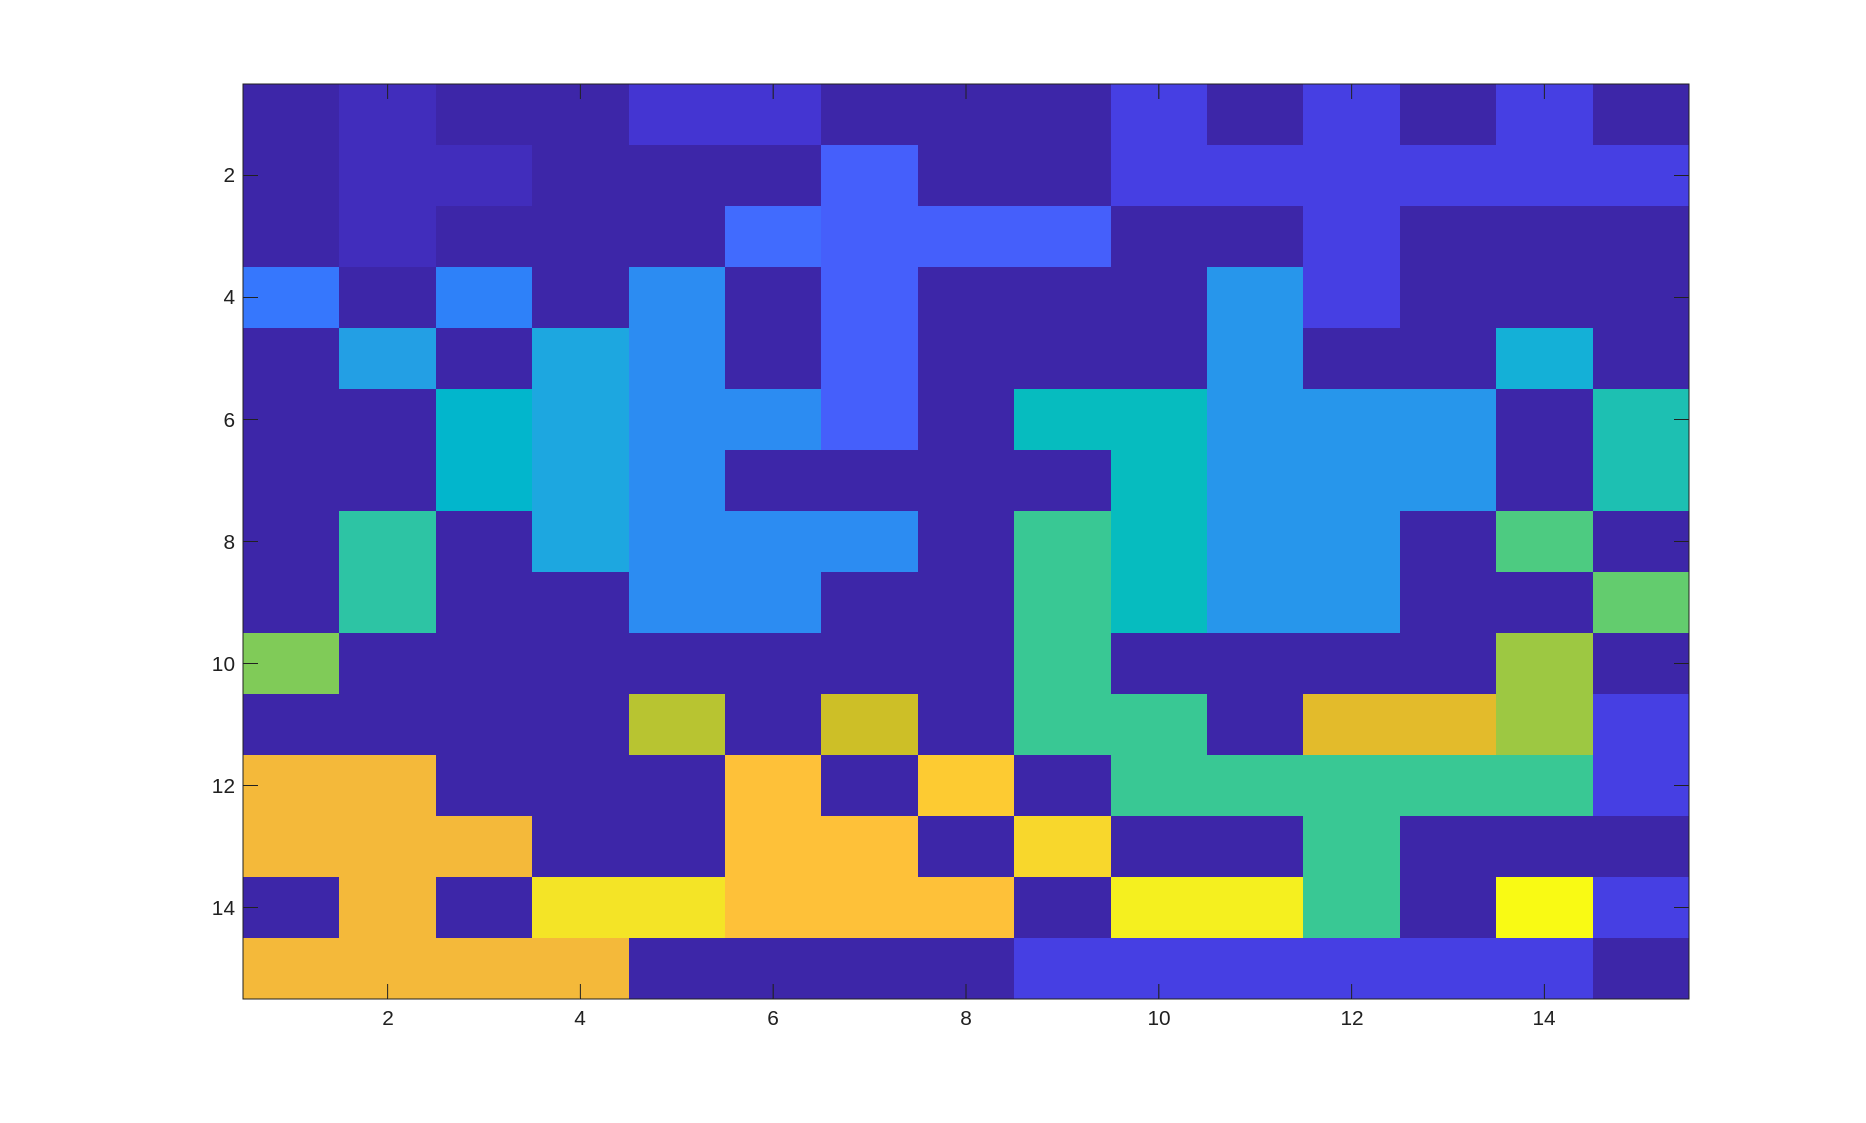
\includegraphics[width=0.7\linewidth]{images/re-labelled-edge}
	\caption{Esempio di ri-labeling limitato ai bordi del reticolo}
	\label{fig:relabelled-edge}
\end{figure}
\\\\
\noindent
Concludiamo dicendo che l'analisi della correttezza dell'implementazione proposta è stata effettuata non soltanto tramite test individuali sul singolo algoritmo, ma anche attraverso un confronto diretto con l'algoritmo naive presentato a lezione. Nello specifico, è stato generato un reticolo bidimensionale di dimensioni $100 \times 100$, con una probabilità di colorazione dei siti pari al 50\%. Tale reticolo è stato analizzato prima con l'algoritmo naive e successivamente con l'algoritmo HK76, confrontando i risultati ottenuti per la percolazione verticale (top-bottom) e orizzontale (left-right). Questo confronto è stato ripetuto $10.000$ volte, e in tutti i casi i risultati forniti dai due algoritmi sono stati coincidenti. 